\section{Ejercicio 3}

En este ejercicio nos piden programar la tarea \textbf{TaskBach} que recibe dos parámetros: \textit{total\_cpu} y \textit{cant\_bloqueos}. La misma debe realizar \textit{cant\_bloqueos} llamadas bloqueantes en momentos elegidos pseudo aleatoriamente y, en cada una de esas llamadas debe permanecer bloqueada durante dos ciclos de reloj. El tiempo de CPU total utilizado debe ser el de \textit{total\_cpu} ciclos de reloj.

Para que esta tarea tenga el comportamiento pedido, lo que hacemos contar cual es la cantidad de tiempo que se va a utilizar el CPU de la siguiente forma:

\begin{center}
		int \textit{cpu\_restante} = \textit{total\_cpu} - \textit{cant\_bloqueos} - 1;
\end{center}

Cada llamada bloqueante utiliza un ciclo de reloj y la función \textbf{return} también utiliza un ciclo. Por ende, los ciclos restantes son los que utilizamos para hacer la llamada a la función \textbf{uso\_CPU}.

Luego, tenemos el siguiente ciclo:

\begin{algorithmic}

\While{\emph{cant\_bloqueos}$> 0$}
	\State Genero un número pseudoaleatorio entre cero y \textit{cpu\_restante} con la función \textbf{rand()}.
	\If{\emph{Si el número generado es mayor que cero}}
		\State Utilizo el CPU ese número generado de clocks.
	\EndIf
	\State Le resto a \textit{cpu\_restante} el número generado.
	\State Llamo a la función \textbf{uso\_IO} con dos clocks.
	\State Le resto uno a \textit{cant\_bloqueos}
\EndWhile
\end{algorithmic}
~
De esta forma, vamos a obtener llamadas bloqueantes en momentos elegidos pseudo aleatoriamente.

Generamos y ejecutamos el siguiente lote, y luego graficamos la simulación usando el algoritmo FCFS con un costo de 3 clocks para cambiar de contexto.

\begin{center}
	\begin{tabular}{|l|}
		\hline
		TaskBatch 23 1		\\
		@5: 				\\
		TaskBatch 42 2		\\
		@6:					\\
		TaskBatch 58 3		\\
		@8:					\\
		TaskBatch 77 4		\\
							\\
		TaskBatch 33 12		\\
		@2:					\\
		TaskBatch 50 5		\\
		@3:					\\
		TaskBatch 70 9		\\
		@2:					\\
		TaskBatch 27 3		\\
		\hline
	\end{tabular}
\end{center}

\begin{figure}[!h]
	\begin{center}
		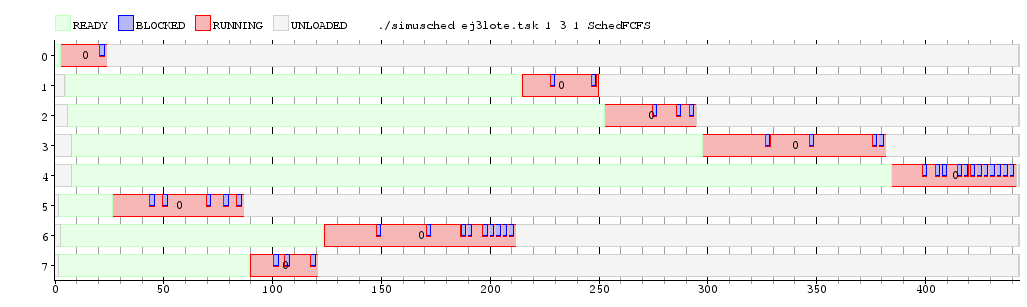
\includegraphics[width=500px]{imagenes/ej3.png}
		\caption{\small{\textbf{Gráfico generado con el lote.}}}
		\label{fig:grafico_ej1}
	\end{center}
\end{figure}
